\documentclass{article}

\usepackage{utf8-math}   % use unicode symbols in tex source
\usepackage[english]{babel}
\usepackage[textsize=small,
%            disable, 
            color={orange!30}, 
            shadow, 
            prependcaption]{todonotes}
\usepackage{stmaryrd}             %\boxempty and ⟦ command
\usepackage{xspace} % correct spacing after operators
\usepackage{floatrow}
%\usepackage{accents} % used for double-hat, double-tilde macro
\usepackage{amsmath}
\usepackage{amsthm}

\usepackage{enumerate}
\usepackage{cancel}
\usepackage{microtype}

\usepackage{tikz}
\usetikzlibrary{arrows, matrix, shapes.misc, decorations, decorations.pathreplacing, automata}

%\usepackage{pgfplots}
\usepackage{tikz-timing}

\usepackage{thmtools}
\usepackage{thm-restate}
\usepackage{listings}
\usepackage[lighttt]{lmodern}
%\usepackage{lmodern}

%\usepackage{hyperref}
%\usepackage{cleveref}

\usepackage{fancyhdr}


\title{TESSLA---A Temporal Stream-based Specification Language}
\newcommand{\thetitle}{TESSLA---A Temporal Stream-based Specification Language}
\title{\thetitle}

\newtheorem{theorem}{Theorem}
\newtheorem{proposition}[theorem]{Proposition}
\newtheorem{definition}[theorem]{Definition}

\pagestyle{fancy}
\setlength{\headheight}{15pt}
\fancyhead[RO]{\thepage}
\fancyhead[LO]{\thetitle}
\fancyfoot[C]{}

\tikzset{
  ampersand replacement=\&, % alternative to using fragile frames
  event/.style = {draw, cross out, inner sep = 1pt,xshift=0.75pt},
  event label/.style = {font = \tiny, label distance = -2pt}  
}


%\renewcommand{\ttdefault}{pcr}

\newcommand{\lstcomment}[1]{\color{darkgray}\rmfamily\scriptsize#1}
\lstset{}
%\lstset{
%%   basicstyle=\ttfamily\scriptsize,
%   basicstyle=\ttfamily\small,
%%   basicstyle=\fontfamily{pcr}\selectfont\small,
%%   keywordstyle=\bfseries\ttfamily\underbar,%
%%   keywordstyle=\fontfamily{pcr}\selectfont\bfseries,
%   keywordstyle=\sffamily\bfseries,
%   columns=fullflexible,
%%    columns=flexible,
%   comment=[l]//,
%   commentstyle=\color{darkgray}\rmfamily\scriptsize,
%   emph={square}, 
%   emphstyle=\color{blue}\textrm,
%   emph={[2]root,base},
%   emphstyle={[2]\color{yac}\textrm},
%   showstringspaces=false,
%%   flexiblecolumns=false,
%   tabsize=3,
%   numbers=left,
%   numberstyle=\tiny,
%   numberblanklines=false,
%   stepnumber=1,
%   numbersep=3pt,
%%   xleftmargin=5pt,
%   %keywords={in, while, foreach, val, var, procedure, proc, fun, function, case, if, then, else, return},
%   aboveskip=3pt,
%   belowskip=3pt,
%%   escapechar=\&
%   escapeinside={*@}{@*} % useful to put a \label in there
% }


\lstset{
%  extendedchars=true,
%  inputencoding=utf8
  basicstyle=\small\ttfamily,
%  stringstyle=
%  keywordsyle={[2]\underbar},
  commentstyle=\rmfamily\it,
  extendedchars=true,
  keepspaces=true, 
  columns=flexible,
  frame=tlrb,
  keywordstyle=\ttfamily\bfseries
}

\lstdefinestyle{long}{}

\lstdefinestyle{inline}{   
  basicstyle=\ttfamily\footnotesize,
  numbers=none,
  xleftmargin=2em,
  aboveskip=0.3ex,
  belowskip=0ex,
%  belowcaptionskip=0em,
%  lineskip=0em
}

\lstdefinelanguage{salt}{
  keywords={always, next, until, not, and, or, implies, if, then},
%  keywordstyle=\rmfamily\it,
  comment=[l]{--}
}

\lstdefinelanguage{tessla}{
  keywords={on, if, define, yield, out, trigger, while, window, and, or},
  keywordstyle=\ttfamily\bfseries,
  classoffset=1,
  morekeywords={EStream,VStream,Int,Bool},  
%  keywordstyle=\ttfamily\bfseries,
  keywordstyle=\underline,
  classoffset=0,
  comment=[l]{--}
}

\lstdefinelanguage{tessla+salt}{
  language=tessla,
%  classoffset=1,
  morekeywords={always, next, until, not, and, or, implies, if, then},
%  keywordstyle=\ttfamily\bfseries,
%  keywordstyle=\underline,
%  classoffset=0,
  comment=[l]{--}
}


%%% Todonotes %%%
\newcommand{\idea}[2][]{\todo[color={blue!15!green!7},nolist, #1]{#2}}
%\newcommand{\idea}[2][]{}
\newcommand{\ignore}[1]{}
%\newcommand{\inappendix}[2][]{\todo[color={yellow!50},nolist,inline #1]{\underline{Appendix} #2}}
\newcommand{\todoil}[1]{\todo[nolist, inline]{#1}}

\newcommand{\defeq}{\mathrel{\texttt{:=}}}


\begin{document}

\maketitle

\section{Introduction}

%Outline
%
%\begin{enumerate}
%  \item purpose, motivation
%  \begin{itemize}
%    \item online processing of data
%    \item monitoring of trace properties, specifically execution traces of programs
%    \item Functional reactive programming as related concept
%  \end{itemize}
%  \item What you describe with a \tessla specification
%  \begin{itemize}
%    \item input, output streams
%    \item application of functions, composition of function
%    \item
%  \end{itemize}
%  \item Modelling data in terms of streams
%  \begin{itemize}
%    \item timing model ($ℝ$,$ℕ$,$ℚ$,…), restrictions to streams with discrete set of time stamps (event streams) or peace-wise constant streams (continuous stream)
%    \item continuous streams and event streams
%   \end{itemize}
%   \item Functions on streams and desired properties (in general)
%   \begin{itemize}
%     \item small examples
%     \item causality, statefulness, time invariance
%     \item (composition lemmata)
%   \end{itemize}
%   \item \tessla syntax
%   \begin{itemize}
%      \item base grammar with functions and type annotations
%      \item syntactical extensions: infix operators, named arguments, the “on”
%   \end{itemize}
%   \item Types
%   \begin{itemize}
%     \item Generic types
%     \item Coercion
%   \end{itemize}
%   \item Functional semantics of operators, small examples
%   \item Larger example/case study
%   \begin{itemize}
%     \item producer/consumer, ring buffer, …
%   \end{itemize}
%
%
%\end{enumerate}


%Purpose of \tessla.

%\begin{itemize}
%  \item analysis of trace data
%  \item specification of failure patterns, correctness properties, transformations
%  \item intuitive, pragmatic means of formulation
%\end{itemize}

%Purpose of this document.
%\begin{itemize}
%  \item Motivate and describe the language
%  \item reference
%  \item case study and examples from the targeted application area
%  \item description of how to integrate runtime verification methodology based on tessla and its implementation into the development process
%\end{itemize}

%Approach
%  \begin{itemize}
%    \item online processing of data
%    \item monitoring of trace properties, specifically execution traces of programs
%    \item Functional reactive programming as related concept
%  \end{itemize}

\subsection{The Setting}

\tessla is developed in the scope of the CONIRAS project as a language for specifying properties of multicore systems. The goal is to observe the execution of C programs on multicore systems with the processor's debug interfaces and check if these executions fulfill a certain correctness property specified in \tessla. The correctness properties are synthesized as a monitor on an FPGA which also gets the data from the debug interfaces. Then the FPGA can check by using the monitor if the properties are violated of satisfied.

The workflow for creating a monitor from a \tessla specification and to monitor a C program is given in Figure \ref{fig:workflow}. At first the observable points, called tracepoints, have to be extracted from the compiled C code with debug symbols. Tracepoints can be various lines in the assembler code, for example jumps, a write to a variable or similar things. These tracepoints are needed in \tessla specifications to relate to certain lines in the C code and thus they are also needed for the \tessla-compiler such that it knows which lines of code in the C program can be observed when they are reached during execution. After a \tessla specification is compiled the compiler outputs a directed acyclic graph (DAG) which contains all the functions and constants used in the specification. Afterwards, this DAG is synthesized on the FPGA to work as a monitor. The data which the monitor works on comes from the debug interfaces of the CPU. Besides the information about which operation was executed, the data contains timestamps and an ownership ID which relates to the core that executed the operation. But before giving the data into the monitor engine on the FPGA the tracepoints have to be reconstructed. Therefore an Instruction Reconstruction (IR) unit is synthesized on the FPGA in front of the monitor engine, hence all data that comes out of the CPU debug interface first goes through this IR unit. The IR unit matches the incoming data to the tracepoints and sends an event to the monitor engine every time a tracepoint was executed by the CPU. All the data that does not related to a tracepoint or does not contain general important information will be filtered out by the IR unit to reduce the amount of data that reaches the monitor.

\begin{figure}
	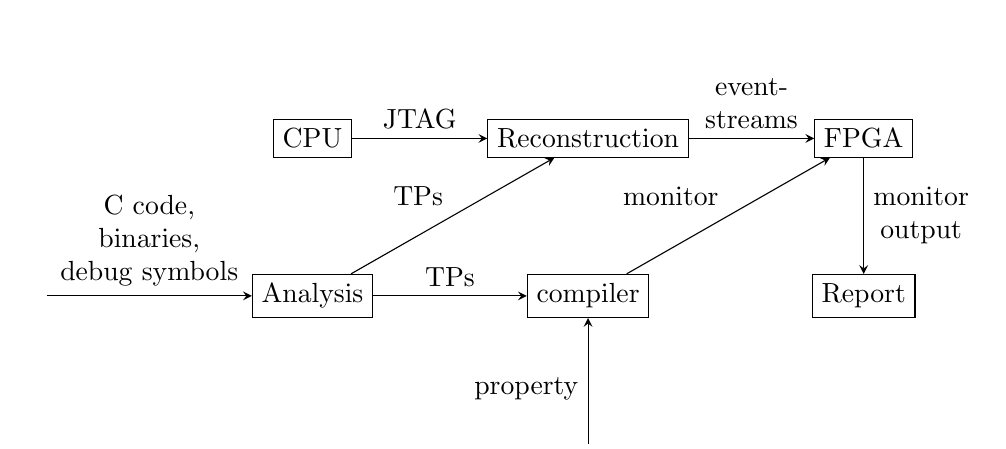
\begin{tikzpicture}[node distance = 3.5cm, on grid = true, auto]

\node[rectangle, draw](cpu){CPU};
\node[rectangle, draw, right of = cpu](reconstruction){Reconstruction};

\node[rectangle, draw, below of = cpu, node distance = 2cm](analysis){Analysis};
\node[rectangle, draw, below of = reconstruction, node distance = 2cm](compiler){\tessla compiler};
\node[left of = analysis, node distance = 3.5cm](c){};
\node[below of = compiler, node distance = 2cm](prop){};
\node[rectangle, draw, right of = reconstruction](fpga){FPGA};
\node[rectangle, draw, below of = fpga, node distance = 2cm](report){Report};

\draw[-stealth]
(cpu) edge node[above]{JTAG} (reconstruction)	
(analysis) edge node[above]{TPs} (compiler)
(c) edge node[align = center]{C code, \\ binaries, \\ debug symbols} (analysis)
(analysis) edge node[above left]{TPs} (reconstruction)
(prop) edge node[align = center, left]{\tessla \\ property} (compiler)
(compiler) edge node[above left]{monitor} (fpga)
(reconstruction) edge node[align = center]{event- \\ streams} (fpga)
(fpga) edge node[align = center]{monitor \\ output} (report)
;

\end{tikzpicture}
	\caption{The workflow for reconstructing the program sequence and synthesizing the monitor for a \tessla specification. The blue nodes represent the part needed for the compilation of a \tessla specification, the red node represents the multicore CPU, the green nodes represent the parts that are synthesized on the FPGA and the orange node represents the output of the verification process. \label{fig:workflow}}
\end{figure}

\subsection{The Design of \tessla}

\subsubsection{General Requirements}

Various requirements lead to the form \tessla has now. Some requirements directly result from setting: because the clock speed of the FPGA is much lower than the one of the CPU cores, an asynchronous processing of the incoming data is necessary which leads to the model of asynchronous streams used in \tessla. Furthermore, the fact that the systems under scrutiny are multicore systems and hence data comes from multiple core in arbitrary order and amount fits the model of asynchronous streams well.

\subsubsection{Timing Requirements}

Besides the requirements that result directly from the setting, there are different requirements which come from the properties that should be specifiable. By viewing the TIMMO specification language used in the AUTOSAR project it becomes clear that real time constraints are really important in the scope of multicore systems. Additionally the difference of the timestamps of two events can be arbitrarily small which leads to the need of a continuous time model with the constraint that in a finite time frame only a finite number of events, and thus timestamps, can occur. Otherwise no monitoring is possible because an infinite number of events has to be processed in a finite amount of time.

Among others these include properties like the following:

\begin{enumerate}
	\item \textit{Every time an event $e_1$ occurs, at most $n$ seconds after (before respectively) $e_1$ another event $e_2$ has to occur.}
	\item \textit{For every event in the event stream $E_1$, at most $n$ seconds after (before respectively) an Event has to occur on the stream $E_2$. Every event that occurs on $E_2$ can only be matched to at most one from $E_1$.}
\end{enumerate}

This results in functions being available in \tessla that work on real time units.

\subsubsection{Arithmetic Requirements}

Other important properties of program executions on CPUs require to count events that are happening and also to apply different arithmetic operations on the counted values. This is needed to recognize buffer overflows, check fairness properties on, for example, variables access or resource usage, prove constraints on the number of function calls in the C code and other properties. Another use case for arithmetics is to make calculations on variable values, for example medians.

Among others these include properties like the following:

\begin{enumerate}
	\item \textit{The difference of the number of write events and the number of delete events for a buffer of size 5 should never exceed 5.}
	\item \textit{The median of the ten last values a temperature sensor delivers should never exceed 20.}
\end{enumerate}

These are typical properties that are interesting for the industry and hence to be able to specify those properties, \tessla needs arithmetic functions.

\subsubsection{Stream Operation Requirements}

Not only but also because of the necessity of counting events, it is necessary to apply operations directly on the input streams. These can transform the data of the events of an input stream or can even add or take out whole events. Typical examples for these operations are if-then constructs or filter and merge functions which are needed in \tessla.

Among others these include properties like the following:

\begin{enumerate}
	\item \textit{There exists a system with three cores. Both core one and core two should be able to access a certain resource at least once every ten seconds.}
	\item \textit{A certain threshold value should not be exceeded by a variable more than three times in the last ten values of that variable.}
\end{enumerate}

\subsubsection{Temporal Logic Requirements}

Besides the properties that are mentioned above an important class of properties is missing: the properties that are specifiable with typical temporal logics such as the LTL or SALT. These have proven to be interesting in a lot of systems. Furthermore the different semantics available for such logics are needed to detect final output values and to detect those as soon as possible such that errors are acknowledged very early. To be able to use those logics it has to be possible to transform formulas of these logics into state machines which leads to the need to detect where such logics are used. Because of this it is the easiest way to include them into \tessla in a separated function. Another positive side effect is that state machines can be synthesized and executed extremely efficient on the FPGA monitor engine.

Properties for which temporal logics can be used are the following:

\begin{enumerate}
	\item \textit{When the only process that writes values to the buffer is deactivated, no write operations should happen on the buffer until the process is activated again.}
	\item \textit{Every time $a$ occurs a $b$ has to be occurred 2 to 5 seconds before.}
\end{enumerate}

\subsection{What you describe with a \tessla specification}

\tessla is conceptually based on streams as a model for data processing and data analysis.
The data to be analysed is considered as input streams and a \tessla specification essentially describes a set of output streams and how they can be derived from the input.
To this end, new streams can be defined by applying some function to existing ones.
For example, given an input stream of integral values, a \tessla specification could describe the stream that consecutively provides the sum of all previous input values.
This is achieved by applying a corresponding function to the input stream and thereby defining a new output stream.

\subsection{Stream Model}
\label{sec:streams}

\begin{figure}
  \input{fig_streams}
  \caption{Example streams.\label{fig:streams}}
\end{figure}

The streams used in \tessla specifications model the essential aspects found in computer programs, namely values (e.g., the value of a program variable), events (e.g., the call of a specific function) and time, both, in a qualitative (ordering) and quantitative (duration) sense.

The timing model is based on time stamps $t∈𝕋$ where we assume $𝕋$ to be isomorphic to the real numbers $ℝ$.\footnote{Notice that we deliberately choose \emph{the continuum} as a model of real time as is common in philosophy, physics and engineering. For our purposes of specifying timing property, however, also a weaker notion of density would clearly suffice, such as the rational numbers $ℚ$.}
Although on the technical level time is mostly quantised in actual systems, real time is a common and intuitive model.
In fact, neither specification nor evaluation based on single steps of, e.g., the a CPU core are reasonable.
Time is therefore handled, formally and technically, in terms of intervals.
In the following, we make the notion of streams precise that provide the semantic basis of the language.
We use $𝕋$ to denote the time domain to make an explicit distinction between time stamps and, e.g., real values.
This avoids confusion and inconsistencies since the representation of time values is implementation dependent.
For example, the values may be scaled according to the processing clock speed and therefore adding or comparing a value $t∈𝕋$ with some real value $r∈ℝ$ is not well defined unless considering a specific execution platform with fixed parameters.
However, we use common operators and symbols to work with time stamps, such as $+$ (addition), $≤$ (ordering) and $0$ (neutral element of addition), that are defined as expected.

We consider two types of streams.
Values, e.g., of a program variable or stored at some specific memory address, might change over time but can be assumed to always be present.
They are represented by continuous streams that we call \emph{signals}. \todo{adde preliminary definitions somewhere, e.g., appendix: piece-wise constant function, segments, intervals, left/right-closed, change points}

\begin{definition}[Signals]
  Let $D$ be a set of data values.
  A \emph{signal of type $D$} is a function $σ: 𝕋_{≥0} → D$ such that
  \begin{itemize}
    \item $σ$ is piece-wise constant,
    \item every segment $I∈\mathsf{seg}(σ)$ is left-closed\footnote{
          A \emph{segment} of a piece-wise constant function $σ: 𝕋_{≥0} → D$ is a maximal interval $I⊂𝕋$ with constant value $v∈D$, i.e., $∀_{t∈I}:σ(t)=v$.} and
    \item the set of change points $Δ(σ) := {\min I|I∈\mathsf{seg}(σ)}$ is discrete\footnote{A subset $M$ of $𝕋$ is \emph{discrete} if it does not contain bounded infinite subsets.}.
  \end{itemize}
  The set of all signals $σ: 𝕋_{≥0} → D$ is denoted $𝓢_D$.
\end{definition}

Apart from values that are conveniently modeled to be continuously available, discrete \emph{events}, like function calls, are of interest.
These are modelled by the second type of streams \emph{event streams} that provide values (events) only at specific points in time wheras no information about the time between two consecutive events is available.

\begin{definition}[Event streams]
  For a set $D$ of data values an \emph{event stream of type $D$} is a partial function $η: 𝕋_{≥0} ⇁ D$ such that the domain of definition, called the set of \emph{event points} $E(η) := \{t∈𝕋|η(t)∈D \text{ defined}\}$, is discrete.
%
  The set of all event streams $η: 𝕋_{≥0} ⇁D$ is denoted $𝓔_D$.
\end{definition}

For convenience we may write $η(t) = ⊥$ to denote that $η$ is not defined at time point $t∈𝕋∖ E(η)$.
To model streams of events that do not carry a value we use a designated type \texttt{Unit}.
Formally, we let $\mathtt{Unit}={⊤}$ be a set with one designated element $⊤$.

The discreteness condition reflects the property of actual systems that time stamps cannot converge because only a bounded number of events can happen within a fixed time period.

In addition to the definition in terms of partial functions, an event stream $η∈𝓔_D$ can be naturally represented as a (possibly infinite) sequence $s_η=(t_0,η(t_0))(t_1,η(t_1))…∈(E(η)×D)^∞$ ordered by time ($t_i<t_{i+1}$ for $0≤i<|s_η|$) and containing all event points (i.e, ${t|(t,v) \text{ occurs on } s_η}= E(η)$).

\subsection{Defining Streams}

\tessla allows for defining streams through function applications.
Such functions can be applied to signal and event streams, as well as constant values.
For example, addition of two (value) streams can be defined as element-wise addition of the values of two signals \texttt{s1} and \texttt{s2}:
\begin{lstlisting}[language=tessla]
  define sum := add(in1, in2)
\end{lstlisting}
Here, $\mathtt{add}: 𝓢_ℕ × 𝓢_ℕ → 𝓢_ℕ$ is a function that maps a pair of signals $\mathtt{in1},\mathtt{in2}∈𝓢_ℕ$ with data domain $ℕ$ to the signal representing their sum at every point in time, i.e.,  $\mathtt{sum}(t) = \mathtt{add}(\mathtt{in1}, \mathtt{in2})(t) = \mathtt{in1}(t) + \mathtt{in2}(t)$ for any time point $t∈𝕋$.

The specification above hence describes a rather simple transformation of two input streams into one output stream.

Regarding evaluation it is reasonable to restrict the functions on streams that can be used in \tessla, depending on their application context.

\begin{definition}[Causality, state, time invariance]
Let $A,B$ be sets of signals or event streams.
A function $f: A → B$ is considered to \emph{respect weak causality} if there is a constant $k∈𝕋$ such that $f(σ)(t)$ is independent of the values $σ(t')$ for $t'>t+k$:
for all $t∈𝕋$ and all $σ,σ'∈A$ we require that $f(σ)(t) = f(σ')(t)$ if $σ(t')=σ'(t')$ for all $t'<t+k$.

The function $f$ is called \emph{stateless} if for all $t∈𝕋$ and all $σ,σ'∈A$ we have $f(σ)(t) = f(σ')(t)$ if $σ(t) = σ'(t)$.

A stateless function $f$ is called \emph{time invariant} if $σ(t) = σ(t')$ implies that $f(σ)(t) = f(σ)(t')$ for all $σ∈A$ and all $t∈𝕋_{≥0}$.
\end{definition}


\idea[inline]{
Example: Detecting a delayed action

Assume the control of a device is supposed to react on an input signal within a specific time bound of 10 microseconds.
The control program receives a signal when the function \texttt{rcv()} is called, needs to process the data and react by calling a function \texttt{react()}.
Given means to observe function calls during the execution of the program\footnote{We will discuss observation approaches in Section~\ref{sec:observation}.} a \tessla specification can be used to formulate the timing constraint.
The calls to \texttt{rcv()} and \texttt{react()} can be considered as input event streams \texttt{rcv} and \texttt{react}.

}

\subsection{Monitoring Engine}

The \tessla\ compiler translates a specification into a DAG of functions.
This DAG is then synthesized on an FPGA in order to execute such a specification.
On the FPGA both signals and event streams are represented
as tuples of data and timestamps.
In case of signals each value change corresponds to such a tuple.
On the FPGA data and timestamps are transferred through seperated lines
with sufficient bus with.
Data and the corresponding timestamp are always kept in sync.
An $n$-ary function in the DAG is translated into a function block with $n$ data inputs,
one timestamp input, one data output and one timestamp output.
Note that every function block has only one timestamp input,
which may require additional synchronization in front of it:
If you want to combine $n$ not yet synchronized streams in one function block,
a synchronization block is added which takes $n$ value inputs and the corresponding $n$ timestamp inputs
and has $n$ value outputs and only one timestamp output.
This block buffers the incoming values and timestamps until all values for a common timestamp are known,
and then emits one timestamp together with $n$ values.
% TODO: Does this hold for signals and event streams? Can we compute new event streams out of multiple event stream? How?


\section{Syntax}

This section describes the syntax of \tessla.

\subsection{Basic Syntax}

As basic syntactic elements of \tessla we consider a set of \emph{types} $T$, \emph{names} $\mathcal{N}$ and \emph{function symbols} $\mathcal{F}$.
Formally, the latter are two families $\mathcal{N}=(N_t)_{t \in T}$ and $\mathcal{F}=(F_{(t_1…t_m)t_{m+1}})_{t_1…t_{m+1} \in T^+}$ of distinct sets of symbols that correspond to a specific type or signature, respectively.
We refer to the tuple $Σ=(T,\mathcal{N}, \mathcal{F})$ as a \emph{signature} providing the basic syntactical elements of our specification language.

Built from those we define \emph{terms} $x$ of type $t \in T$ and sequences of terms $seq$ by the grammar
\[\begin{array}{rl}
x &::= n \mid f_c \mid f(seq) \mid x : t\\
seq &::= x \mid x,seq
\end{array}\]
where $n \in N_t$, $f_c \in F_{()t}$ (i.e., constants) and $f \in F_{(t_1…t_m)t}$.

\subsection{Syntactical Extensions}

We consider three syntactical extensions to the base syntax presented above. The first is an \emph{on} operator, the second are \emph{infix operators} and the third are \emph{named arguments}.

Let us consider the \emph{on} operator first. Therefore, for a set of function symbols $F_{(t_1…t_m)t}$ let $F^s_{(t_1…t_m)t} \subseteq F_{(t_1…t_m)t}$ be the set of function symbols of stateless functions. Hence the \emph{terms} $x$ of a type $t \in T$ including the \emph{on} operator can be defined by the grammar
\[\begin{array}{rl}
x &::= n \mid f_c \mid f(seq) \mid \operatorname{on} f_s(seq_s) \mid x : t\\
seq &::= x \mid x,seq \\
y &::= n \mid f_c \mid f_s(seq_s) \mid \operatorname{on} f_s(seq_s) \mid y : t \\
seq_s &::= y \mid y,seq_s
\end{array}\]
where $f_s \in F^s_{(t_1…t_m)t}$ and the rest is defined as before.

\textcolor{red}{TODO: !infix operators, named arguments!}

\section{Semantics}

In this section, the semantics of \tessla is defined. All in all, the functions used in \tessla can be categorized in six different types. Before we start with the semantics of the function we will fix some notation first.

In the following we will use $\mathcal{S},\mathcal{C}$ and $\mathcal{E}$ for the sets of all streams, continuous streams and event streams, respectively. With $\mathcal{C}[T]$ we refer to the set of continuous streams that only contain elements of the type $T$ (f.e. $\mathcal{C}[\mathbb{B}]$ is the set of continuous boolean streams). We will use $\mathbb{D}$ as the set of all values.

Furthermore we will use the function $\operatorname{prev}: \mathcal{C} \times \mathbb{Q} \rightarrow \mathcal{C}$ to refer to the value that was on the stream prior to a certain time stamp, which is defined as follows:

\[\operatorname{prev}(c,t) = n \text{ with } \exists t' < t: c(t') = n \land \nexists t' < t'' < t: c(t'')\not= n \]  

\subsection{Arithmetic Functions}

Arithmetic functions take a certain number of value streams of type integer and return a stream that contains either integer or boolean values. The semantics for the arithmetic functions are defined in the following.

The function $\operatorname{add}: \mathcal{C}[\mathbb{N}] \times \mathcal{C}[\mathbb{N}] \rightarrow \mathcal{C}[\mathbb{N}]$ for adding the values of two integer streams is defined as follows:

\[\operatorname{add}(n_1,n_2) = n_3 \text{ with } n_3(t) = n_1(t) + n_2(t)\]

The function $\operatorname{sub}: \mathcal{C}[\mathbb{N}] \times \mathcal{C}[\mathbb{N}] \rightarrow \mathcal{C}[\mathbb{N}]$ for subtracting the values of the second integer stream from the value of the first integer stream is defined as follows:

\[\operatorname{sub}(n_1,n_2) = n_3 \text{ with } n_3(t) = n_1(t) - n_2(t)\]

The function $\operatorname{mul}: \mathcal{C}[\mathbb{N}] \times \mathcal{C}[\mathbb{N}] \rightarrow \mathcal{C}[\mathbb{N}]$ for multiplying the values of two integer streams is defined as follows:

\[\operatorname{mul}(n_1,n_2) = n_3 \text{ with } n_3(t) = n_1(t) \cdot n_2(t)\]

The function $\operatorname{geq}: \mathcal{C}[\mathbb{N}] \times \mathcal{C}[\mathbb{N}] \rightarrow \mathcal{C}[\mathbb{B}]$ for checking if the values of the first integer stream is at least as big as the value of the second integer stream is defined as follows:

\[\operatorname{geq}(n_1,n_2) = b_1 \text{ with } b_1(t) = n_1(t) \geq n_2(t)\]

The function $\operatorname{leq}: \mathcal{C}[\mathbb{N}] \times \mathcal{C}[\mathbb{N}] \rightarrow \mathcal{C}[\mathbb{B}]$ for checking if the values of the first integer stream is at least as big as the value of the second integer stream is defined as follows:

\[\operatorname{leq}(n_1,n_2) = b_1 \text{ with } b_1(t) = n_1(t) \leq n_2(t)\]

The function $\operatorname{equals}: \mathcal{C}[\mathbb{N}] \times \mathcal{C}[\mathbb{N}] \rightarrow \mathcal{C}[\mathbb{B}]$ for checking if the values of two integer streams are equal is defined as follows:

\[\operatorname{equals}(n_1,n_2) = b_1 \text{ with } b_1(t) = \begin{cases}
\text{true} & \text{if } n_1(t) = n_2(t) \\
\text{false} & \text{else}
\end{cases}\]

The function $\operatorname{max}: \mathcal{C}[\mathbb{N}] \times \mathcal{C}[\mathbb{N}] \rightarrow \mathcal{C}[\mathbb{N}]$ for getting the maximum of the current values of two integer streams is defined as follows:

\[\operatorname{max}(n_1,n_2) = n_3 \text{ with } n_3(t) = \begin{cases}
n_1(t) & \text{if } n_1(t) > n_2(t) \\
n_2(t) & \text{else}
\end{cases}\]

The function $\operatorname{min}: \mathcal{C}[\mathbb{N}] \times \mathcal{C}[\mathbb{N}] \rightarrow \mathcal{C}[\mathbb{N}]$ for getting the minimum of the current values of two integer streams is defined as follows:

\[\operatorname{max}(n_1,n_2) = n_3 \text{ with } n_3(t) = \begin{cases}
n_1(t) & \text{if } n_1(t) < n_2(t) \\
n_2(t) & \text{else}
\end{cases}\]

The function $\operatorname{not}: \mathcal{C}[\mathbb{B}] \rightarrow \mathcal{C}[\mathbb{B}]$ for getting the negation of the value of a boolean stream is defined as follows:

\[\operatorname{not}(b_1) = b_2 \text{ with } b_2(t) = \neg b_1(t)\]

The function $\operatorname{or}: \mathcal{C}[\mathbb{B}] \times \mathcal{C}[\mathbb{B}] \rightarrow \mathcal{C}[\mathbb{B}]$ for combining two boolean streams with an or is defined as follows:

\[\operatorname{or}(b_1, b_2) = b_3 \text{ with } b_3(t) = b_1(t) \lor b_2(t)\]

\subsection{Timing Functions}

Timing functions take a certain number of continuous streams and return a continuous or event stream. The semantics for the timing functions are defined in the following.

The function $\operatorname{delay}: \mathcal{C} \times \mathbb{Q} \rightarrow \mathcal{C}$ for delaying the values of the input stream for a certain amount of time is defined as follows:

\[\operatorname{delay}(c_1,q) = c_2 \text{ with } c_2(t) = c_1(t - q)\]

The function $\operatorname{getTimestamp}: \mathcal{C} \rightarrow \mathbb{Q}$ for replacing the values of the input stream with its timestamps is defined as follows:

\[\operatorname{getTimestamp}(c_1) = c_2 \text{ with } c_2(t) = t\]

The function $\operatorname{inPast}: \mathcal{C} \times \mathbb{D} \times \mathbb{Q} \rightarrow \mathcal{C}[\mathbb{B}]$ for checking if a certain value holds in a given time frame in the past is defined as follows:

\[\operatorname{inPast}(c_1, d, q) = b \text{ with } b(t) = \begin{cases}
\text{true} & \text{if } \exists t - q \leq t' \leq t: c_1(t') = d \\
\text{false} & \text{else}
\end{cases}\]

The function $\operatorname{synchronize}: \mathcal{C} \times \mathcal{C} \times \mathbb{Q} \rightarrow \mathcal{E}$ for checking whether a corresponding event occurs in the second stream for each event in the first stream within a certain time frame is defined as follows:

\[\operatorname{synchronize}(c_1,c_2,q) = e_1 \text{ with } e_1(t) = \begin{cases}
\top & \text{if } c_1(t - q) = x_i \land \forall t-q \leq t' \leq t: c_2(t') \not= y_i \\
\bot & \text{else}
\end{cases}\]

\textcolor{red}{$x_i$ bzw. $y_i$. Is there a better way?}

\subsection{Aggregations}

Aggregation functions take a certain number of continuous streams and return an continuous integer stream. The semantics for the aggregation functions are defined in the following. \textcolor{red}{second input / reset still missing!}

The function $\operatorname{maximum}: \mathcal{C}[\mathbb{N}] \rightarrow \mathcal{C}[\mathbb{N}]$ for computing the maximum of all values that occurred on the stream is defined as follows:

\[\operatorname{maximum}(n_1) = n_2 \text{ with } \forall t' < t: n_2(t) \geq n_1(t') \land \exists t' < t: n_2(t) = n_1(t')\]

The function $\operatorname{minimum}: \mathcal{C}[\mathbb{N}] \rightarrow \mathcal{C}[\mathbb{N}]$ for computing the minimum of all values that occurred on the stream is defined as follows:

\[\operatorname{minimum}(n_1) = n_2 \text{ with } \forall t' < t: n_2(t) \leq n_1(t') \land \exists t' < t: n_2(t) = n_1(t')\]

The function $\operatorname{sum}: \mathcal{C}[\mathbb{N}] \rightarrow \mathcal{C}[\mathbb{N}]$ for computing the sum of all values that occurred on the stream is defined as follows:

\[\operatorname{sum}(n_1) = n_2 \text{ with } ???\]

The function $\operatorname{eventCount}: \mathcal{S} \rightarrow \mathcal{C}[\mathbb{N}]$ for computing the number of Events that occurred on the stream is defined as follows:

\[\operatorname{eventCount}(s_1) = n_1 \text{ with } ???\]

\subsection{Selectors/Filters/Conditionals/Combinators}

The function $\operatorname{ifThen}: \mathcal{C}[\mathbb{B}] \times \mathcal{C} \rightarrow \mathcal{C}$ for returning the value of the second input stream if the value of the first stream is true is defined as follows:

\[\operatorname{ifThen}(b_1,c_1) = c_2 \text{ with } c_2(t) = \begin{cases}
c_1(t) & \text{if } b_1(t) \\
\operatorname{prev}(c_2,t) & \text{else}
\end{cases}\]

The function $\operatorname{ifThenElse}: \mathcal{C}[\mathbb{B}] \times \mathcal{C} \times \mathcal{C} \rightarrow \mathcal{C}$ for returning the value of the second input stream if the value of the first stream is true and the value of the third input stream otherwise is defined as follows:

\[\operatorname{ifThenElse}(b_1,c_1,c_2) = c_3 \text{ with } c_3(t) = \begin{cases}
c_1(t) & \text{if } b_1(t) \\
c_2(t) & \text{else}
\end{cases}\]

The function $\operatorname{merge}: \mathcal{C} \times \mathcal{C} \rightarrow \mathcal{C}$ for merging two streams is defined as follows:

\[\operatorname{merge}(c_1,c_2) = c_3 \text{ with } ???\]

\subsection{Monitors}

The monitor function can be used to enable the usage of temporal logics within \tessla. A monitor takes a temporal logic formula and returns an output value that depends on the evaluation status of the given formula at the current point in time. Let TL be a temporal logic, $\varphi \in \operatorname{TL}$ a formula of TL and $\llbracket . , . \rrbracket_{\operatorname{TL}}: \operatorname{TL} \times \mathbb{Q} \rightarrow \mathcal{C}$ be the function that returns the truth value of $\varphi$ at a certain point in time. Then the semantics of the function $\operatorname{monitor}: \operatorname{TL} \rightarrow \mathcal{C}$ is given as follows:

\[\operatorname{monitor}(\varphi) = c_1 \text{ with } c_1(t) = \llbracket \varphi, t \rrbracket_{\operatorname{TL}}\]

\subsection{On}

\section{Recursion in \tessla}

Currently, there is no possibility to define a stream recursively, hence with a reference to its previous value. There are two functions \texttt{delay} and \texttt{shift} which are intended for delaying a stream by a certain amount of time or shifting the data values of events of an event stream by a certain number of events. These functions look as if they can be used for recursive stream definitions but in most cases this does not work as expected. This is the reason why functions like \texttt{synchronize}, \texttt{eventCount} or the calculation of a sum by using \texttt{sum} are atomic functions which leads to the problem that a user can not define his own functions when recursive calls are needed for the definition.

To solve this problem, a function \texttt{last} is needed that works quiet similar to \texttt{shift} and \texttt{delay}, but has some important differences. Over event streams the function $\texttt{last}: 𝓔_D \rightarrow 𝓢_D$ is defined as follows:
\[\texttt{last}(\eta)(t) = \eta(t') \Leftrightarrow t' \in E(\eta) \land t' < t \land \nexists t' < t'' < t: t'' \in E(\eta)\] 

Over signals the function $\texttt{last}: 𝓢_D \rightarrow 𝓢_D$ is defined as follows:
\[\texttt{last}(\sigma)(t) = \sigma(t') \Leftrightarrow t' \in E(\texttt{changeOf}(\sigma)) \land t' < t \land \nexists t' < t'' < t: t'' \in E(\texttt{changeOf}(\sigma))\] 

This new function allows us to define streams recursively, for example, \texttt{synchronize}, \texttt{eventCount} and \texttt{sum} can be defined as follows:

Count events recursively:
\begin{lstlisting}[language=tessla+salt]
define eventCount(x) := onYield(x, last(eventCount(x)) + 1
\end{lstlisting}

Build a sum recursively:
\begin{lstlisting}[language=tessla+salt]
define sum(x) := onYield(x, last(sum(x))) + mrv(x)
\end{lstlisting}

Build a synchronization recursively:

\begin{lstlisting}[language=tessla+salt]
define diff_x := eventCount(delay(x,2s)) - last(eventCount(err_x)) - 
  (eventCount(y) - last(eventCount(err_y)))
define err_x := filter(on(changeOf(diff_x)), diff_x > 0)

define diff_y := eventCount(delay(y, 2s)) - last(eventCount(err_y)) - 
  (eventCount(x) - last(eventCount(err_x)))
define err_y := filter(on(changeOf(diff_y)), diff_y > 0)

out occurAny(err_x, err_y)
\end{lstlisting}

\appendix

\section{Examples}

\tessla specification formally describe transformations of input to output streams where the set of input streams is defined implicitly by names occurring freely in the specification. 
In practice, however, a more specific control over the inputs is desired and therefore implementations may provide specific input functions, that only depend on constants, e.g., strings describing the stream source.

In the following examples we assume input functions
\begin{align*}
 \mathtt{function\_calls}&: \mathtt{String} → 𝓔_D\\
 \mathtt{function\_returns}&: \mathtt{String} → 𝓔_D
\end{align*}
Similarly, the representation of time (intervals) is implementation dependent.
In the example specification we use integer numbers and suffixes (us,ms,s) to indicate appropriate factors. 
Ideally, an implementation will convert, e.g.,  $1s$, $1ms$ and $1us$, into a representation of 1 second, 1 millisecond and 1 microsecond, respectively.

Double hyphens (\texttt{--}) indicate commentary until line ending.

\subsection{Delay}

Property: Whenever an event \emph{source\_event} occurs, within the next 1.2 seconds the next event \emph{target\_event} must occur.
A \emph{target\_event} can serve for multiple \emph{source\_event} occurrences.

\subsubsection{Delay using SALT}

\begin{lstlisting}[language=tessla+salt]
define source_event := function_calls("main.c:open_door")
define target_event := function_returns("main.c:open_door")

define monitor_output := monitor("always (if p1 then next timed[<= 1200] p2)", sourc_event, target_event)

-- define monitor_output := monitor("always (if {source_event} then next timed[<= 1200] target_event)")

out monitor_output
\end{lstlisting}

%\subsubsection{Delay with SALT and macros}
%
%\begin{lstlisting}
%define delay_constraint(source, target, bounds) :=
%    monitor(always (if {source} then next timed[bounds] target))
%
%out delay_constraint(on entry open_door, on exit close_door, <= 1200)
%\end{lstlisting}

\subsubsection{Delay using SALT without real time operators}

\begin{lstlisting}
define source_event := function_calls("main.c:open_door")
define target_event := function_returns("main.c:open_door")

define monitor_output := monitor("always (if p1 then p2), source_event, inFuture(1200ms, target_event))

out monitor_output
\end{lstlisting}

\subsection{Strong Delay and Order}

Property: For every \emph{source\_event} a matching \emph{target\_event} must occur within the next 1.2 seconds.
Every \emph{target\_event} is associated to at most one \emph{source\_event}.

\begin{lstlisting}
define source_event := function_calls("main.c:open_door")
define target_event := function_returns("main.c:open_door")

define event_pairs := synchronize(source_event, target_event, 1200ms)
define error := timeout(event_pairs)

out error
\end{lstlisting}

\subsection{Synchronization}

Property: Whenever an event occurs, all other events have to occur also within a range of 1.2 seconds. 

\subsubsection{Synchronization using SALT}

\begin{lstlisting}
define event_a := instruction_executions("test.c:23")
define event_b := instruction_executions("test.c:42")
define event_c := instruction_executions("test.c:1729")

define monitor_output := monitor("
  always (
    (if p1 then (next timed[<= 1200] p2 or previous timed[< 1200] p2)) and
    (if p1 then (next timed[<= 1200] p3 or previous timed[< 1200] p3)) and
    (if p2 then (next timed[<= 1200] p1 or previous timed[< 1200] p1)) and
    (if p2 then (next timed[<= 1200] p3 or previous timed[< 1200] p3)) and
    (if p3 then (next timed[<= 1200] p1 or previous timed[< 1200] p1)) and
    (if p3 then (next timed[<= 1200] p2 or previous timed[< 1200] p2)))", 
  event_a, 
  event_b, 
  event_c
)

out monitor_output
\end{lstlisting}

\subsubsection{Synchronization using SALT without real time operators}

\begin{lstlisting}
define event_a := on breakpoint test.c:23
define event_b := on breakpoint test.c:42
define event_c := on breakpoint test.c:1729

define monitor_output := monitor(
  "always (
    (if p1 then p5) and
    (if p1 then p6) and
    (if p2 then p4) and
    (if p2 then p6) and
    (if p3 then p4) and
    (if p3 then p5))",
  event_a,
  event_b,
  event_c,
  within(-1200ms, 1200ms, event_a),
  within(-1200ms, 1200ms,event_b),
  within(-1200ms, 1200ms,event_c)
)

out monitor_output
\end{lstlisting}

\subsection{Periodic}

Eigenschaft: Es gibt ein periodisch auftretendes Event (period\_event). Jedes mal, wenn period\_event auftritt, 
muss nach spätestens einer Sekunde ein anderes Event (event) auftreten. Jedes Auftreten von event muss 
allerdings mindestens 0.7s auseinander liegen.

\subsubsection{Periodic mit SALT}

\begin{lstlisting}
define periodic_event := on breakpoint test.c:34653
define event := on breakpoint test.c:242

define monitor_output := monitor(always((if {period_event} then next timed[<= 1000] event) 
	    and (if {event} then not(next timed[< 700] event))))

out monitor_output
\end{lstlisting}

\subsubsection{Periodic mit SALT und Macro}

\begin{lstlisting}
define periodic_event := on breakpoint test.c:34653
define event := on breakpoint test.c:242

define periodic(period,e,jitter,bound) := 
    monitor(always((if {period} then next timed[<= jitter] e) 
	    and (if {e} then not(next timed[< bound] e))))

out periodic(periodic_event,event,1000,700)
\end{lstlisting}


\subsubsection{Periodic mit SALT ohne SALT-Echtzeitoperatoren}

\begin{lstlisting}
define periodic_event := on breakpoint test.c:34653
define event := on breakpoint test.c:242

define monitor_output := monitor(always((if {period_event} then {within([<= 1000],event)}) 
	    and (if {event} then not({within([< 700],event)}))))

out monitor_output
\end{lstlisting}

\subsection{Use Cases D1-D4}

\subsubsection{Use Case D1 - Simple Saftey Constraint}

Assume an input stream, generated by the application. 
Only values from the range 0-10 are supposed to occur.

\begin{lstlisting}
 define error := on changes(APPL_MSG_Value) if APPL_MSG_Value > 10
 out error
\end{lstlisting}

\subsubsection{Use Case D2 - Timing Constraints}

Assume an input (event) streams @A@ and @B@.

* D2.1 Avent @B@ must not occur within 500ms after any occurrence of event @A@. (Notice implicit conversion of Int → Time in terms of milliseconds.)
  
\begin{lstlisting}
  define syncedAB := synchronise(A, B, 500)
  define error21 := when(not(syncedAB.timeout))
\end{lstlisting}

Alternative:
\begin{lstlisting}
  define error21b := A && within([>0 & <500], B)
\end{lstlisting}

Salt (G(A → ¬X^{<=500} B))
\begin{lstlisting}
  define error21c := monitor always if {A} then not next timed [<500ms] {B}
\end{lstlisting}

* D2.2 In the environment of 500ms around every event A some B must occur
\begin{lstlisting}
  define error22 := A && within([>-500 & <500], B)
\end{lstlisting}

\subsubsection{Use Case D3 - Numerical analysis}

Assume input streams @A@ and @B@

* D3.1 Value excceds limit of 1023
\begin{lstlisting}
  define error31 := A > 1023
\end{lstlisting}

* D3.2 Difference between maximum and minium value exceeds limit of 1023
\begin{lstlisting}
  define error32 := max(A) - min(A) > 1023
\end{lstlisting}
With resets: @max(A: Stream[T], rst: Stream[Any]): Stream[T]@


* D3.3 “Standard deviation” of A exceeds limit of 1023
Unbiased estimation of standard deviation:
\begin{lstlisting}
  define error 33 := count(A) > 1  && sqrt( (sum(A**2) - ( (sum(A)**2)/count(A) )) / (count(A)-1)) ) > 1023
\end{lstlisting}
Maximal difference to mean:
\begin{lstlisting}
define error33 := (max(A) - mean(A) > 1023) || (mean(A) - min(A) > 1023)
\end{lstlisting}

* D3.4 Value of A diverges by more than 1023 from moving average of previous 10 values
\begin{lstlisting}
define error34 := when(SMA(A, 10) > 1023)
\end{lstlisting}

h1. Syntax Sugar Beispiele

\subsection{Events}

\begin{lstlisting}
define someEvent := on entry read_file
-- desugars to:
define someEvent := on("entry read_file")
-- expands to:
define someEvent := when(IR_EVT_MSG = eventId("entry read_file"))
--                       ^- HW stream ^- constant value
\end{lstlisting}

Eine event id kann ein beliebiger Bezeichner sein der eine Stelle im rekonstruierten Codefluss darstellt.

\subsection{Monitore}

\begin{lstlisting}
define someOtherProperty := ...
define someProperty := monitor always if {on entry irqHandler} then {someOtherProperty} until {on exit irqHandler}
-- desugars to:
define someProperty := monitor("always if X then Y until Z", X := on entry irqHandler, Y := someOtherProperty, Z := on exit irqHandler)
\end{lstlisting}

\subsection{Parametrisierte Monitor}

Mit <code>foreach X monitor Y</code> kann die eigenschaft Y für jeden wert von X unabhängig überwacht werden. Dies entspricht einem Slicing der Eingabeströme des Monitors anhand von X.

\begin{lstlisting}
define someProperty := foreach threadId monitor always if {watchdogEvent} then next timed[<5s] {watchdogEvent}
-- desugars to
define someProperty := foreachMonitor(threadId, "always if X then next timed[<5s] X", X := watchdogEvent)
\end{lstlisting}

\nocite{*}
% ---- Bibliography ----
\bibliographystyle{alpha}
\bibliography{bibliography}
%\bibliography{references-auto-dblp,references-manual}

\end{document}
